% Stata exports tabular-only bodies (no \begin{table}); this wrapper owns float, caption, label, notes, width.
\providecommand{\ChapterTableNoteText}[1]{\parbox[t]{0.94\textwidth}{#1}}
\providecommand{\InputStataRegTable}[4]{%
\begin{table}[htbp]
\centering
\caption{#1}%
\label{#2}%
\begin{threeparttable}
\small
\resizebox{\textwidth}{!}{%
\input{#3}%
}%
\begin{tablenotes}[flushleft]
\footnotesize
\item \ChapterTableNoteText{#4}%
\end{tablenotes}
\end{threeparttable}
\end{table}%
}
% Tighter layout for wide panel tables.
\providecommand{\InputStataRegTableCompact}[4]{%
\begin{table}[htbp]
\centering
\caption{#1}%
\label{#2}%
\begin{threeparttable}
\begingroup
\footnotesize
\setlength{\tabcolsep}{4pt}%
\renewcommand{\arraystretch}{0.94}%
\resizebox{\textwidth}{!}{%
\input{#3}%
}%
\endgroup
\begin{tablenotes}[flushleft]
\footnotesize
\item \ChapterTableNoteText{#4}%
\end{tablenotes}
\end{threeparttable}
\end{table}%
}

% Constrain very tall tables to both page width and height.
\providecommand{\InputStataRegTableCompactFitPage}[4]{%
\begin{table}[p]
\centering
\caption{#1}%
\label{#2}%
\begin{threeparttable}
\begingroup
\footnotesize
\setlength{\tabcolsep}{3pt}%
\renewcommand{\arraystretch}{0.90}%
\begin{adjustbox}{max totalsize={\textwidth}{0.74\textheight},center}
\input{#3}%
\end{adjustbox}
\endgroup
\begin{tablenotes}[flushleft]
\footnotesize
\item \ChapterTableNoteText{#4}%
\end{tablenotes}
\end{threeparttable}
\end{table}%
}

%%%%%%%%%%%%%%%%%%%%%%%%%%%%%%%%%%%%%%%%%%%%%%%%%%%%%%%%%%%%%%%%%%%%%%%%%%%
\section{Determinants of trust}
\label{sec:appendix}

\par The focus of this paper is the general trust measure. Table~\ref{tab:42_trust_determinants} describes the set of controls and determinants of general trust. The first column includes standard demographics (gender, education, marital status, and race/ethnicity) while the second column adds variables more unique to the 2020 wave of the HRS questionnaire such as hometown population size and the \say{Potential for Deception} measures for social security, medicare/medicaid, banks, financial advisors, mutual funds, and insurance companies. The third column adds health conditions, insurance coverage, life insurance, and marital history. The fourth column repeats that specification and adds an indicator for leaving any bequest. Columns~\textit{(2)--(4)} include census region; columns~\textit{(1)--(4)} include five-year age-bin fixed effects (coefficients omitted to save space). Below the main fit statistics, the table reports Wald tests for the \say{Potential for Deception} block and joint tests for age bins, race/ethnicity, and region where those terms appear in the column.

\InputStataRegTableCompactFitPage{\textbf{Determinants of General Trust}}{tab:42_trust_determinants}{../../Code/Analysis/Tables/42_table1_trust_determinants.tex}{OLS. Heteroskedasticity-robust standard errors. Column~\textit{(1)}: demographics, depression, and labor force. Column~\textit{(2)}: adds population size, wealth deciles, region, born in U.S., and six \say{Potential for Deception} items. Column~\textit{(3)}: adds health conditions, Medicare/Medicaid, life insurance, and marital history. Column~\textit{(4)}: same as column~\textit{(3)} plus an indicator for any bequest. Age-bin fixed effects are included in all columns but omitted from the body of the table. Region is included in columns~\textit{(2)--(4)} only. The footer lists the deception joint $p$-value and joint tests for age, race, and region.}
\FloatBarrier

\par As \cite{Alesina2000} suggests, demographic variables tend to determine trust. In the HRS data, the estimated coefficients for non-Hispanic Black and for marital status have the strongest significance; the race coefficient is negative, consistent with \cite{Alsan2018}. Depression is negative and significant across specifications.

%%%%%%%%%%%%%%%%%%%%%%%%%%%%%%%%%%%%%%%%%%%%%%%%%%%%%%%%%%%%%%%%%%%%%%%%%%%
\section{Measures of income}

\par Labor income is a narrow measure only capturing earnings and unemployment income. Total income is a more broad measure including retirement and capital income. Figure~\ref{fig:income_over_time} shows that, for the time period, mean incomes are relatively flat over the period. Moreover, the discrepancy between mean labor and total income is likely driven by the oversampling of older and retired households by the HRS.

\begin{figure}[H]
\centering
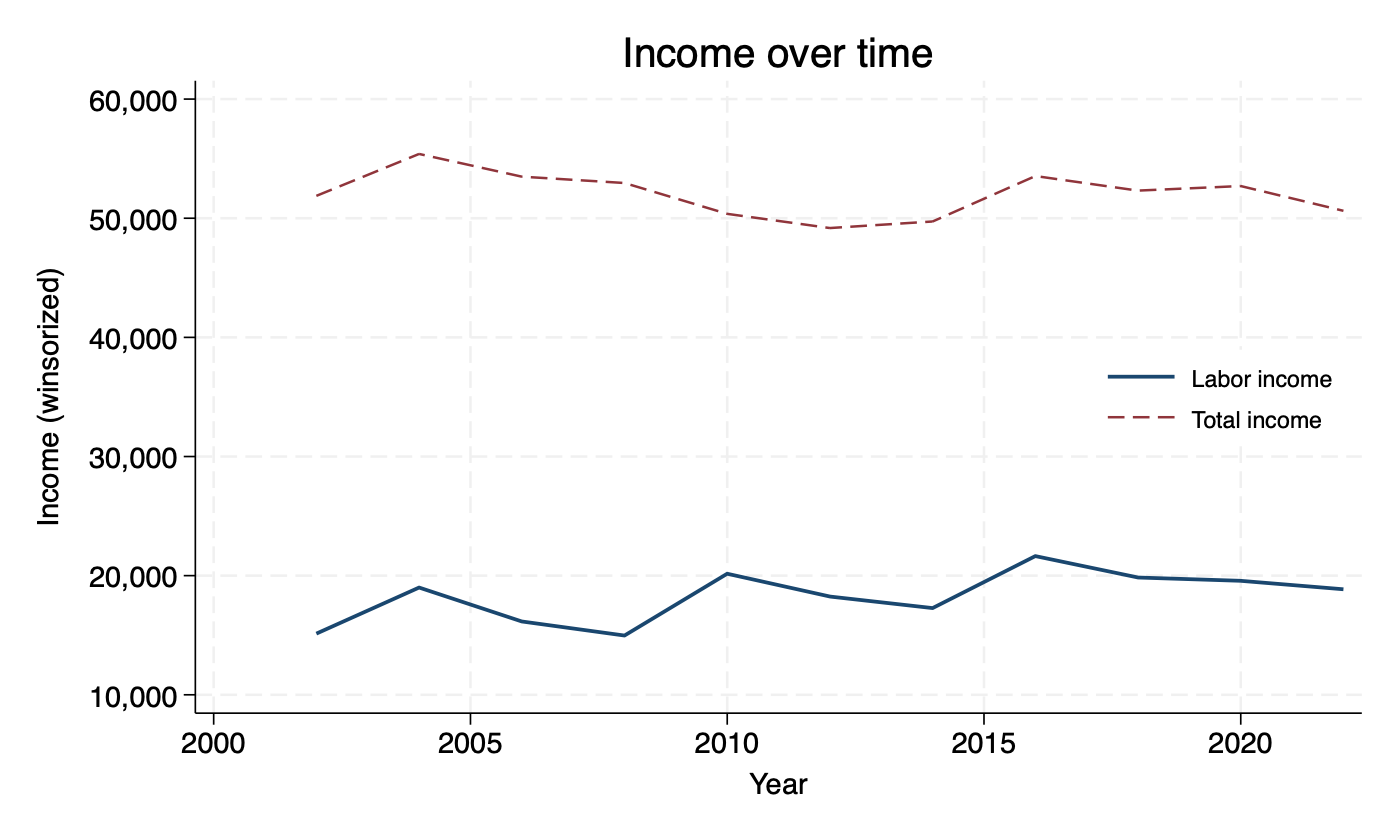
\includegraphics[width=0.8\textwidth]{../../Code/Descriptive/Figures/income_over_time.png}
\caption{Income over time}
\label{fig:income_over_time}
\end{figure}
\FloatBarrier

\par In particular, I pooled the observations of the survey together to get a sense of the distribution of incomes measured in the survey. This is captured by Table~\ref{tab:42_income_tabstat}.

\InputStataRegTableCompact{\textbf{Income Distribution Summary Statistics}}{tab:42_income_tabstat}{../../Code/Analysis/Tables/42_table2_income_tabstat.tex}{Real USD, winsorized; person-years restricted to the same pooled regression sample used for return descriptives in the main text (Tables~\ref{tab:39_r5_age_bin} and~\ref{tab:39_r5_educ_cat}).}
\FloatBarrier

\par An important finding in the literature on earnings in the U.S. is that it is generally hump-shaped over the lifecycle. It is a good sign then that Figure~\ref{fig:income_by_agegroup_2020} displays this pattern.

\begin{figure}[H]
\centering
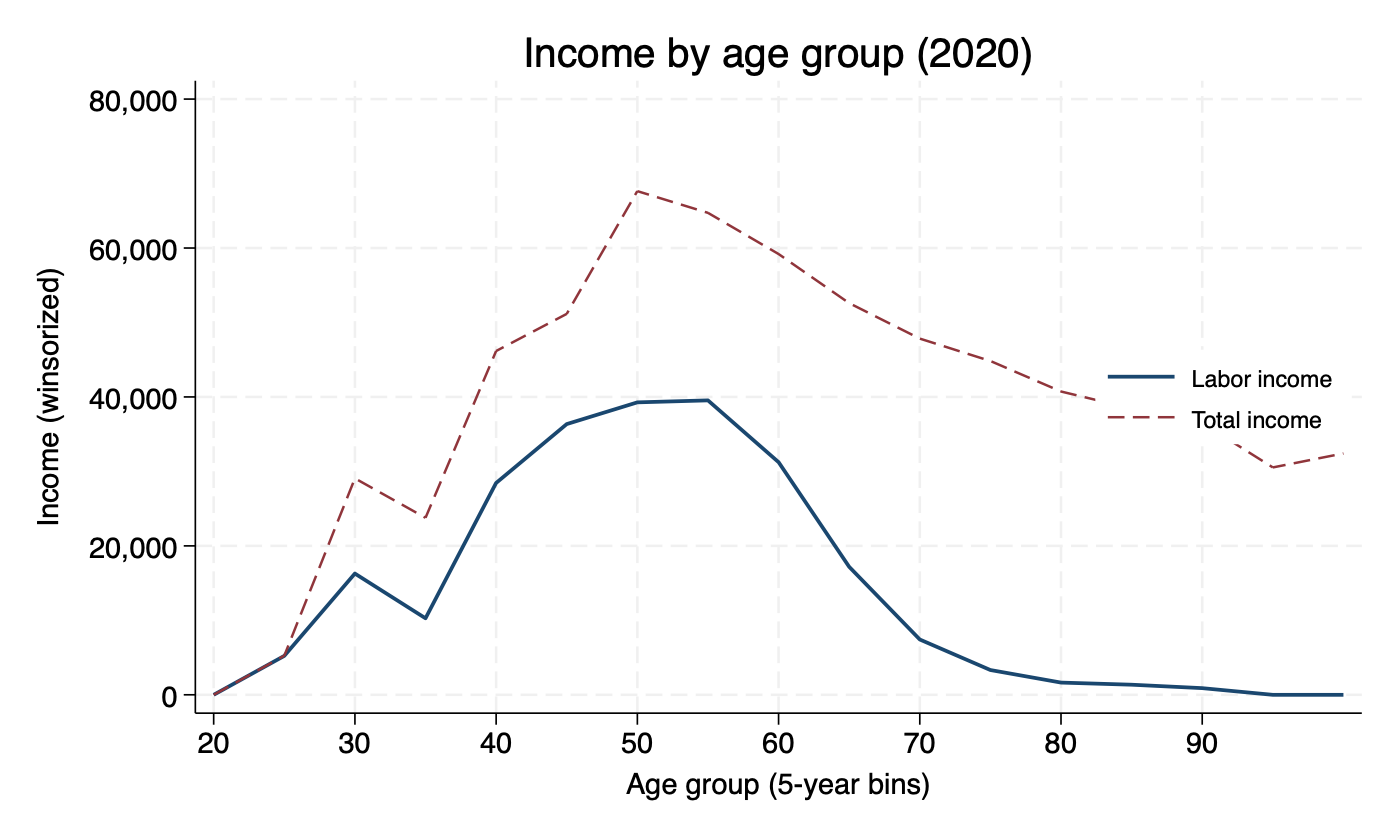
\includegraphics[width=0.8\textwidth]{../../Code/Descriptive/Figures/income_by_agegroup_2020.png}
\caption{Income by age group (2020)}
\label{fig:income_by_agegroup_2020}
\end{figure}
\FloatBarrier

\par Another empirical finding in the literature on earnings is that on average individuals with more education earn higher income. The trend captured in Table~\ref{tab:42_income_by_educ} suggests that the earnings data is in line with what one would expect regarding earnings for a representative survey in the U.S.\footnote{Although the HRS oversamples older households, I use the provided respondent-level weights for this interpretation of the summary statistics of the data.}

\InputStataRegTableCompact{\textbf{Mean Income by Education Group}}{tab:42_income_by_educ}{../../Code/Analysis/Tables/42_table3_income_by_educ.tex}{Real USD, winsorized; same person-year sample as Table~\ref{tab:42_income_tabstat}. No hs $=$ $<$12y; Hs $=$ 12y; Some college $=$ 13--15y; 4yr $=$ 16y; Grad $=$ 17+y.}
\FloatBarrier

\begin{figure}[H]
\centering
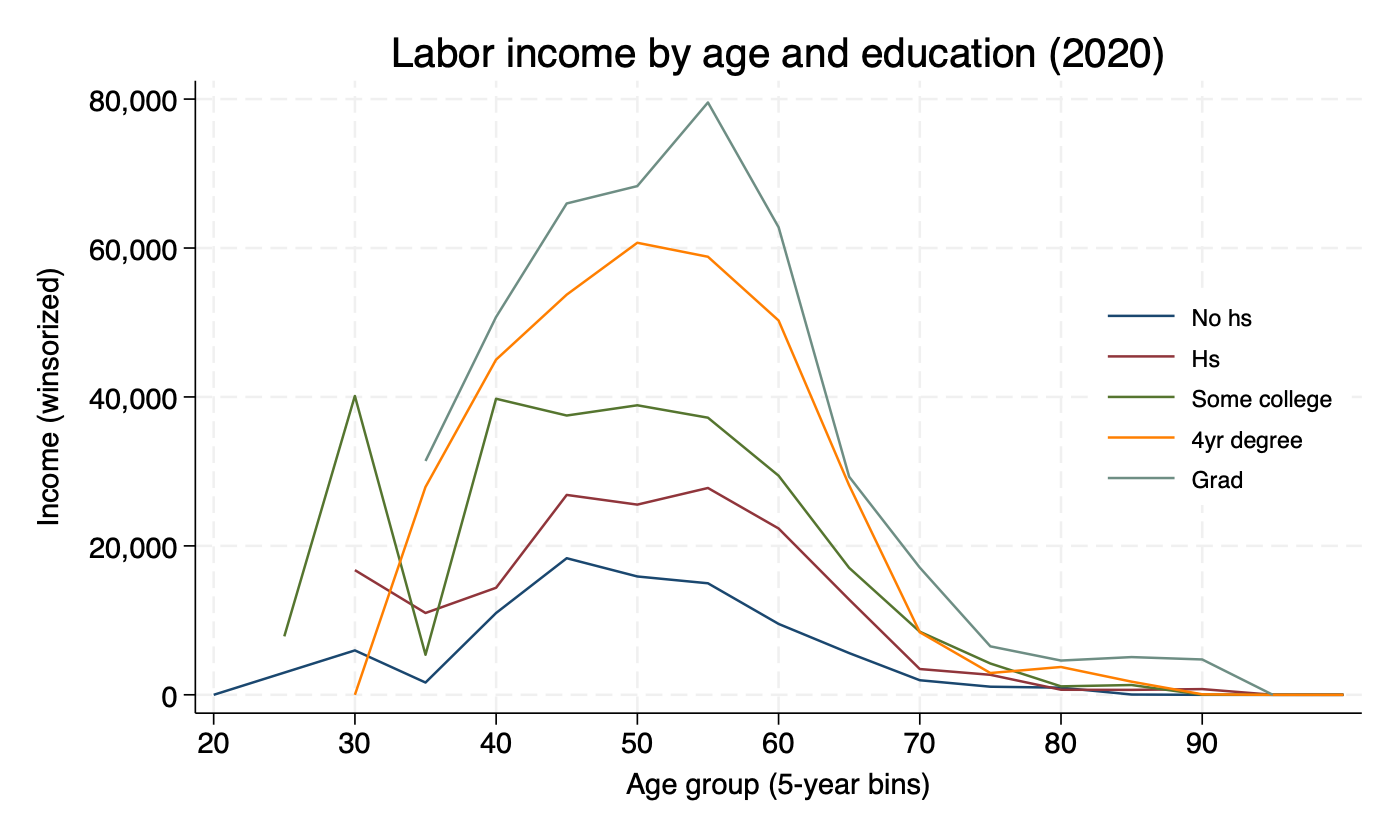
\includegraphics[width=0.8\textwidth]{../../Code/Descriptive/Figures/labinc_by_age_educ_2020.png}
\caption{Labor income by age and education (2020)}
\label{fig:labinc_by_age_educ_2020}
\end{figure}
\FloatBarrier

\begin{figure}[H]
\centering
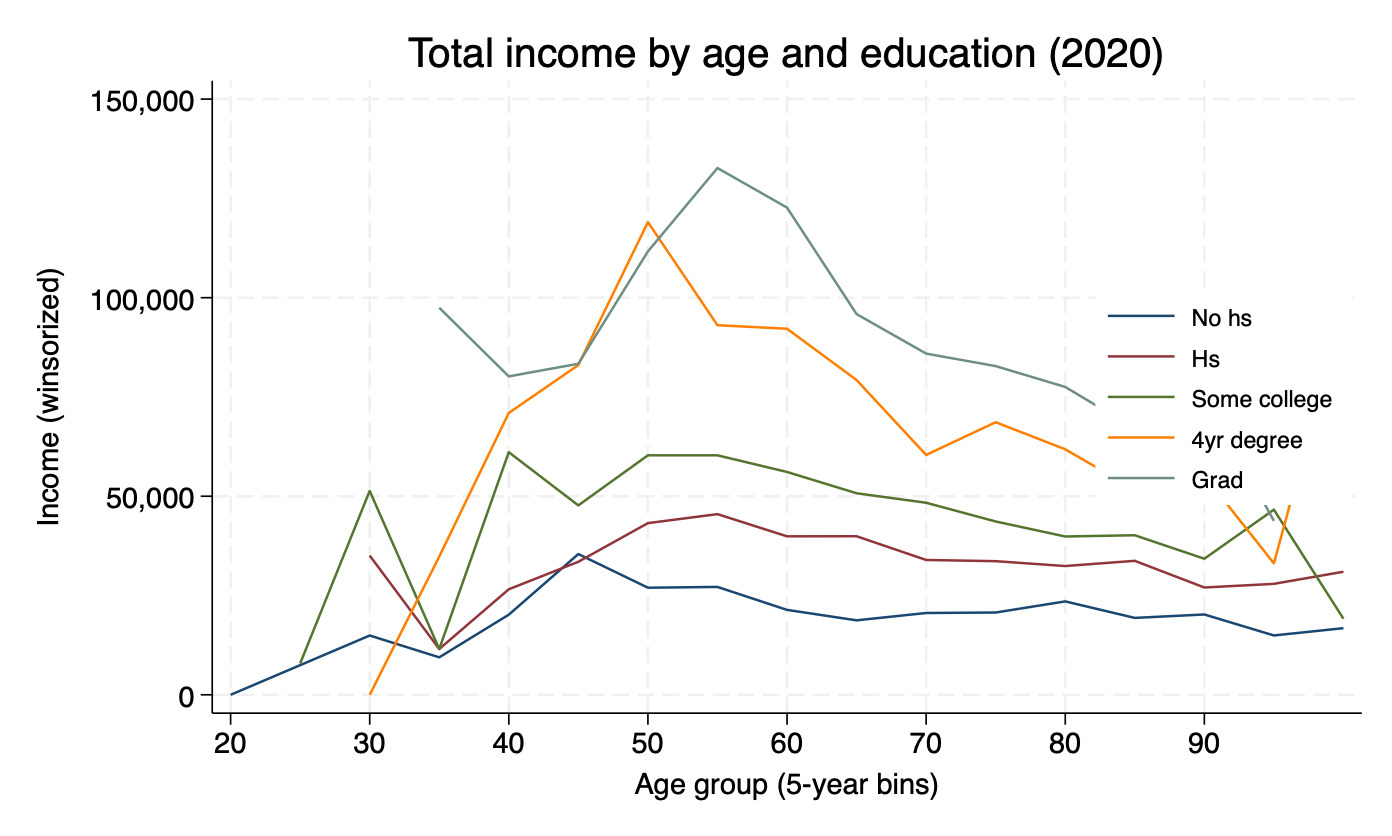
\includegraphics[width=0.8\textwidth]{../../Code/Descriptive/Figures/totinc_by_age_educ_2020.png}
\caption{Total income by age and education (2020)}
\label{fig:totinc_by_age_educ_2020}
\end{figure}
\FloatBarrier

%%%%%%%%%%%%%%%%%%%%%%%%%%%%%%%%%%%%%%%%%%%%%%%%%%%%%%%%%%%%%%%%%%%%%%%%%%%
\section{Trust and total income}

\par This section is an attempt to test whether the hump-shaped relationship between trust and income in \cite{jbpglg2016} holds for the 2020 HRS cohort. I focus the analysis of the empirical relationship between both income and returns and trust on a subset of measures. For income, I omit the analysis for labor income. I also exclude the analysis of the log of total income. Labor income results are not statistically significant. Given the oversampling of older, retired households, lack of predictive power for trust on labor income is not alarming. Total income results are robust to both log and IHS transformations.

\par In Table~\ref{tab:42_income_trust_ihs}, we see the coefficients for both the linear and quadratic terms are significant; the predictive power survives even when the additional controls important for explaining income are included. Since the goal is to uncover whether there is a maximal level of trust regarding economic performance, then we care about the significance of both trust coefficients. Here, we reject the hypothesis that both coefficients are $0$.\footnote{This rejection of the Wald test for the linear and quadratic trust terms (i.e.\ reject both coefficients are zero) will be true for most of the models analyzed in this paper.}

\InputStataRegTableCompact{\textbf{Trust and Total Income (2020)}}{tab:42_income_trust_ihs}{../../Code/Analysis/Tables/42_table4_income_trust_ihs.tex}{Cross-sectional OLS. Heteroskedasticity-robust standard errors. Dependent variable is the inverse hyperbolic sine of deflated, winsorized 2020 total income. Columns~\textit{(1)--(2)}: trust only (linear and quadratic). Columns~\textit{(3)--(4)}: adds age-bin FE, gender, education, labor force, marital status, US birthplace, and race/ethnicity. Age-bin coefficients omitted from display.}
\FloatBarrier

\par I also conduct the joint Wald test for the null hypotheses that the coefficients on the age bins and race categories are jointly equal to zero. In both cases, the null hypothesis is rejected at conventional significance levels.

\par With income data available from 2002--2022, I consider the statistical relationship between average total income and trust. This can be seen in Table~\ref{tab:42_avg_income_trust_ihs}. Not only does the pattern persist, but the significance is stronger not only for trust coefficients, but for the other explanatory variables as well. Again, the Wald tests on the coefficients for race and age bins are rejected, meaning each matter for long-run total income.

\InputStataRegTableCompact{\textbf{Trust and Average Income}}{tab:42_avg_income_trust_ihs}{../../Code/Analysis/Tables/42_table5_avg_income_trust_ihs.tex}{Cross-sectional OLS. Heteroskedasticity-robust standard errors. Dependent variable is the IHS of average total income (deflated, winsorized) over waves 2002--2022. Columns~\textit{(1)--(2)}: trust only (linear and quadratic). Columns~\textit{(3)--(4)}: adds full controls. Age-bin coefficients omitted from display.}
\FloatBarrier
